\documentclass{article}
\usepackage[utf8]{inputenc}
\usepackage{graphicx}
\usepackage{amssymb}

\title{\textbf{Brute-Force String Matching Algorithm}}
\author{Saeah Go}
\date{October 29th 2021}

\begin{document}

\maketitle

\section{\textbf{Abstract}}
\indent \indent The exact string matching problem is to find the occurrences of a pattern of length m from a text of length n symbols. We develop a string-matching problem by brute force algorithm. Brute force is a straightforward approach to solving a problem, usually directly based on the problem statement and definitions of the concepts involved. So the brute force string matching algorithm is just making comparisons for each index of text with the pattern. In the report, the brute force string matching algorithm is presented and analyzed. We will try to visualize the process of string matching and figure out the time efficiency for several cases. We will consider the best, average, and worst cases while comparing the running time for each case. Our experimental results show that the algorithms perform very well in practice. 

\section{\textbf{Introduction}}
\indent We consider several classical string matching problems, given a string of \textit{n} characters called the text $T[0 \ldots n-1]$ and a string of \textit{m} characters (when $m \le n$) called the pattern $P[0 \ldots m-1]$, finding a substring of the text that matches the pattern. So we want to find \textit{i}, the index of the leftmost character of the first matching substring in the text – such that
\begin{center}
$t_i = p_0, \ldots , t_{i+j} = p_j, \ldots , t_{i+m-1} = p_{m-1}$ 
\end{center}
\indent So a brute-force algorithm for the string-matching problem is quite obvious: align the pattern against the first m characters of the text and start matching the corresponding pairs of characters from left to right until either all the m pairs of the characters match(then the algorithm can stop) or a mismatching pair is encountered. In the latter case, shift the pattern one position to the right and resume the character comparisons. We should note that the last position in the text that can still be a beginning of a matching substring is $n-m$ (provided the text positions are indexed from $0$ to $n-1$). The best case is finding the pattern in our first trial. In this case, we only execute m times of loop (to see if text and pattern really match each other), so the time efficiency is $O(m)$. The worst-case happens when we can't find the matching pattern in the text. More specifically, if we have a text like `AAAAAAA' and the pattern is `AAB' then we compare $m(n-m+1)$ times. (When $m \le n$) So in the worst case, the algorithm makes $m(n-m+1)$ character comparisons, which puts it in the $O(nm)$ class. \\
This is how we get $O(nm)$, instead of $O(m(n-m+1)$.
\begin{center}
$O(m(n-m+1))$ \\
$= O(m \times n) (\because{ m \le n})$ \\
$= O(n \times m)$ \\
$= O(nm)$ \\ 
\end{center} 
However, for a typical word search in a natural language text, we should expect that most shifts would happen after very few comparisons. 

\section{\textbf{Background}}
\indent We use the following notation. The text is $T[0 \ldots n-1]$ and the pattern is $P[0 \ldots m-1]$. To show the pattern matches more precisely for the visualization program, we visualize with \textunderscore instead of whitespace. For the visualization part, I tried to show if it's partially matched or fully matched. For the fully matched one, I added to print out ``$\ldots [match]!$" to make sure and show that the given pattern is matched. If the string is partially matched, just print out the partially matched string. If its first letter is not matched (so does not match at all), then print just the first letter. Our goal for this report is looking to verify that the wall clock time performance as the input gets bigger reflects the theoretical complexity class.

\section{\textbf{Data Analysis Process or Procedure}}
\indent We did this experiment with a few cases of small inputs, and we decided to test three different cases (the best, average (random), and worst cases) for each input to show the time complexity. In other words, during the experiment, we moved the matched string locations. We considered three cases for each input: a string only upper cases, a string with only lower cases, and a string with a mixture of upper and lower cases. So we choose to consider the total of five strings, which input sizes are 6, 13, 18, 29, and 37. \\
\indent Not only performance testing, but we also had to measure the time. Timing data is collected by measuring the starting time using time.time() function in the time package. After the searching, we used the time.time() function again to check the time and subtract those to get the execution time. \\
\indent Now let's look at the procedures by checking the test cases one by one.

\subsection{\textbf{Input Size 6}}
\begin{center}
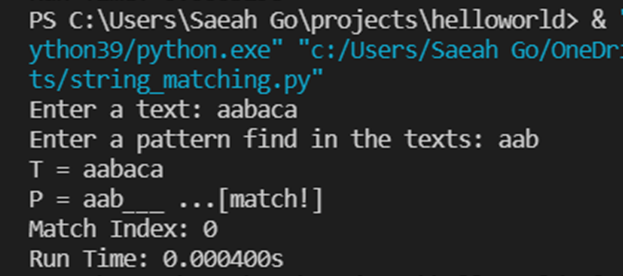
\includegraphics[scale = 0.7]{inputsize 6 best.png} \\
\end{center}
This can be considered as a best case, since the pattern $aab$ was found in the first trial (Match Index zero), which only execute loop $m = 3$ times. 
\begin{center}
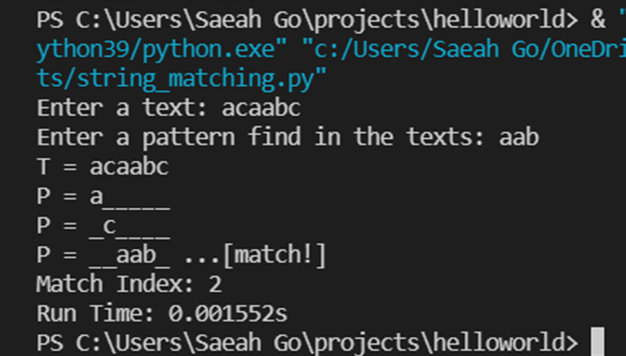
\includegraphics[scale = 0.7]{inputsize 6 average.png} \\
\end{center}
The pattern is matched in the string while executing the loop, but not in the end. Thus this is considered as an average case (or say random case), we can see that the running time is bigger than the best case's running time. ($0.001552s > 0.000400s$) 
\begin{center}
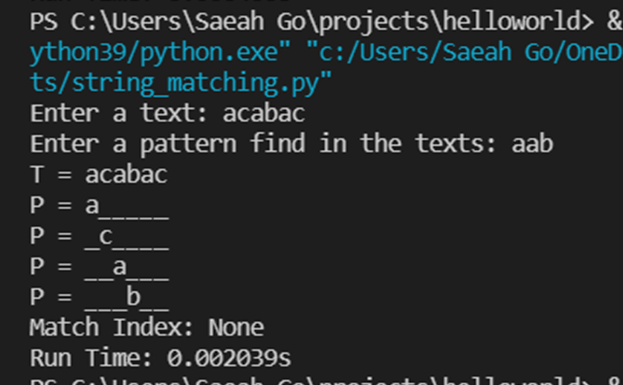
\includegraphics[scale = 0.7]{inputsize 6 worst.png} \\
\end{center}
The given pattern is never matched in the text, so this is the worst case. No matching index exists, and the run time is about 0.02 seconds, we can see it takes more time than the first two cases we tested.

\subsection{\textbf{Input Size 13}} 
\begin{center}
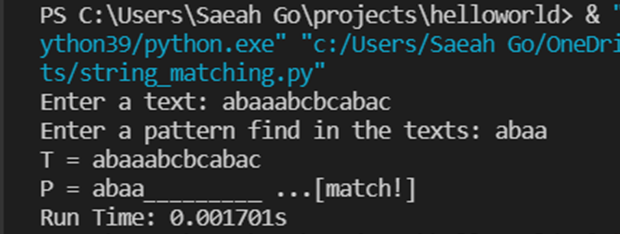
\includegraphics[scale = 0.7]{inputsize 13 best.png} \\
\end{center}
The pattern $abaa$ can be found in our first comparisons, the for loop executed four times, and this is considered as a best case. The execution time is $\approx$ 0.001 seconds, which satisfies our expectation that as the pattern size gets bigger(the pattern size is bigger in this case ($m=4$) than the above case($m=3$)) and thus it takes more time. ($0.001 > 0.0004$)
\begin{center}
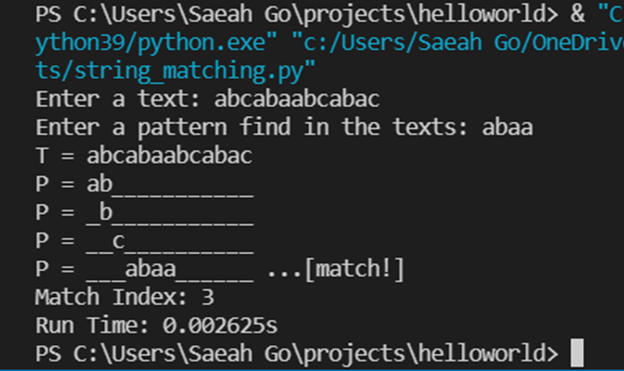
\includegraphics[scale = 0.7]{inputsize 13 average.png} \\
\end{center}
In this average case we got 0.002625 seconds for the execution time, which is bigger than our best case ($0.001701$s) and less than our worst case ($0.004055$s). 
\begin{center}
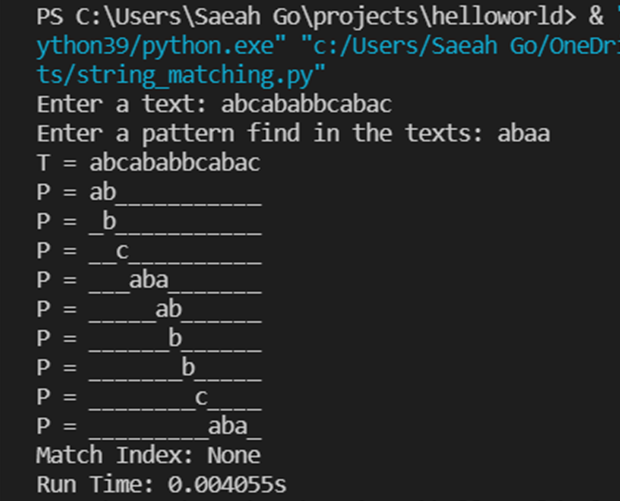
\includegraphics[scale = 0.7]{inputsize13 worst.png} \\
\end{center}
We couldn't find a part that the pattern and the text is matched, so no matching index is found. The execution time for this is $0.004055$ seconds.

\subsection{\textbf{Input Size 18}} 
\begin{center}
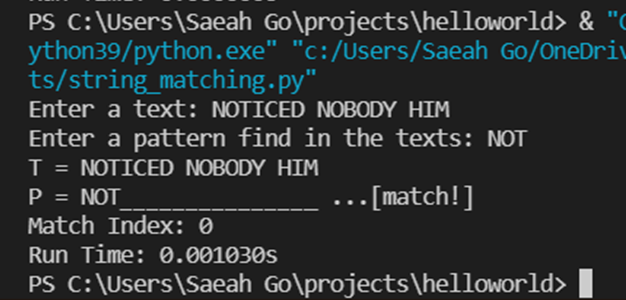
\includegraphics[scale = 0.7]{inputsize 18 best.png} \\
\end{center}
Again, in this case we find the pattern $NOT$ in the comparison when the index $i$ is zero. The execution time is about $0.001$ seconds, which makes sense since we only executed the loop $m=3$ times.
\begin{center}
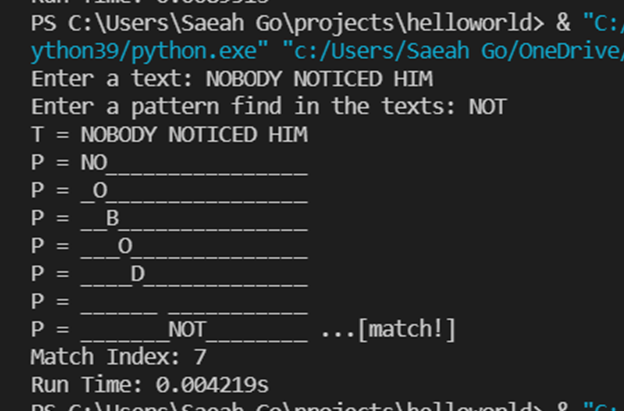
\includegraphics[scale = 0.7]{inputsize 18 average.png} \\
\end{center}
The input size is 18 and the matching index is seven, which means we found the matched string in the middle of the text, not in the first index or last index or couldn't find matching index. So this is a random case, and the random case has approximately $0.004$ seconds of execution time. The running time satisfies our expectation that the running time for the average case is less than the worst case but more than the best case. In this case, best case time execution $\approx 0.001 <$ average (random) case time execution $\approx 0.004 <$ worst case time execution $\approx 0.009$.
\begin{center}
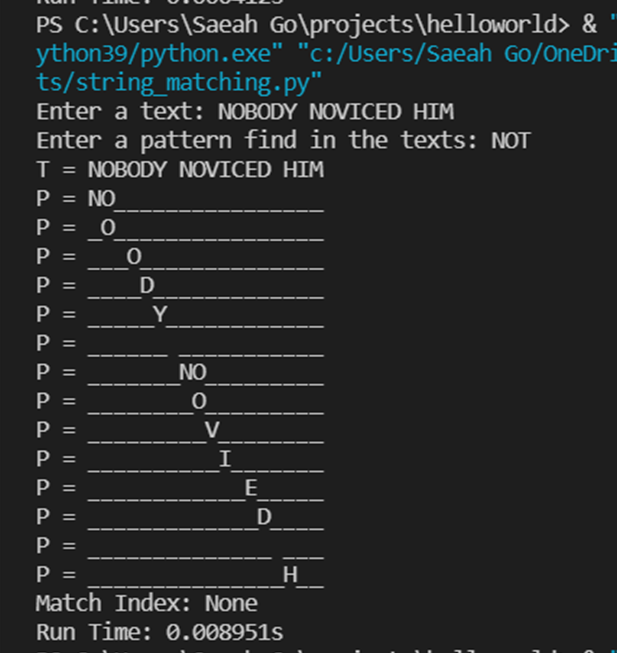
\includegraphics[scale = 0.7]{inputsize 18 worst.png} \\
\end{center}
This is the worst case as we couldn't find the exact matched string pattern in the text. We got $0.008951$ seconds for the execution time, which is much bigger than the best and average cases. We could see that the worst cases time execution is getting much bigger as the input size is larger.

\subsection{\textbf{Input Size 29}} 
\begin{center}
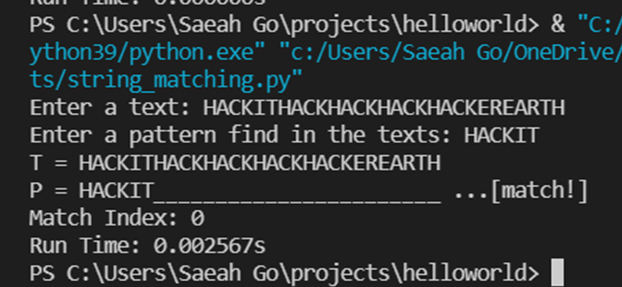
\includegraphics[scale = 0.7]{inputsize 29 best.png} \\
\end{center}
This is another best case, the matching index is zero and we got about $0.002$ seconds for the running time. We could see that the best cases' time execution is not bigger as the input size (text size) increases, since it depends on our pattern size. 
\begin{center}
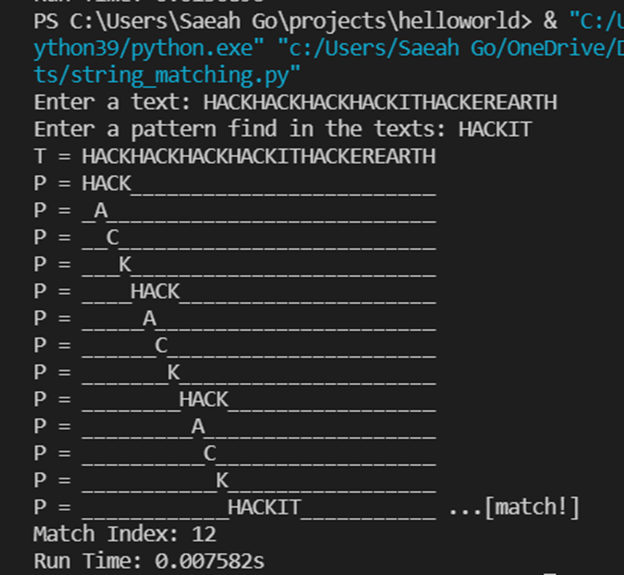
\includegraphics[scale = 0.7]{inputsize 29 average.png} \\
\end{center}
We found the matched string in our $12^{th}$ index from total 29 text sizes, so we found the pattern about the middle of the text. This is the average case and the running time in this case is $0.007582$ seconds.
\begin{center}
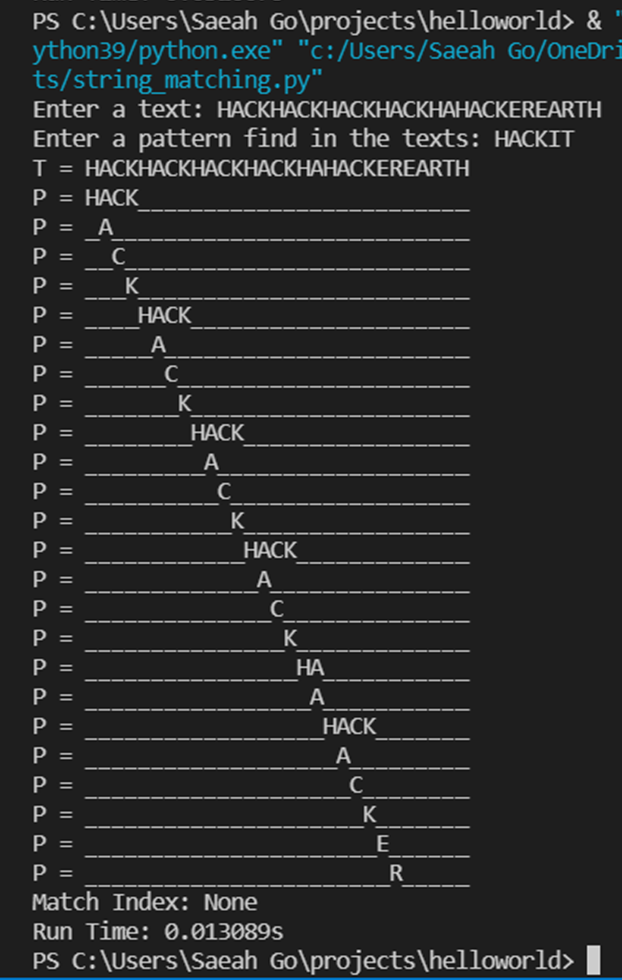
\includegraphics[scale = 0.6]{inputsize 29 worst.png} \\
\end{center}
This is a really long text and we couldn't find our matched pattern in the text. This is considered as a worst case and the execution time for this is $0.013089$ seconds, which is a lot bigger than previous cases.

\subsection{\textbf{Input Size 37}} 
\begin{center}
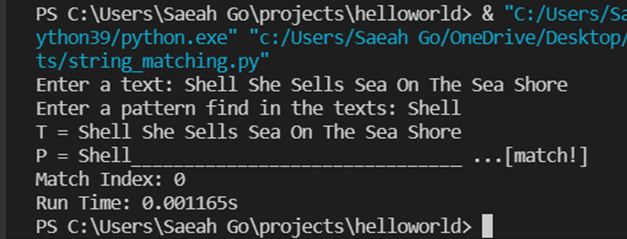
\includegraphics[scale = 0.7]{inputsize 37 best.png} \\
\end{center}
We still got the small running time ($0.001165$ seconds), since our pattern sizes are similar each other and we found the matched string in our first trial in all the best cases. 
\begin{center}
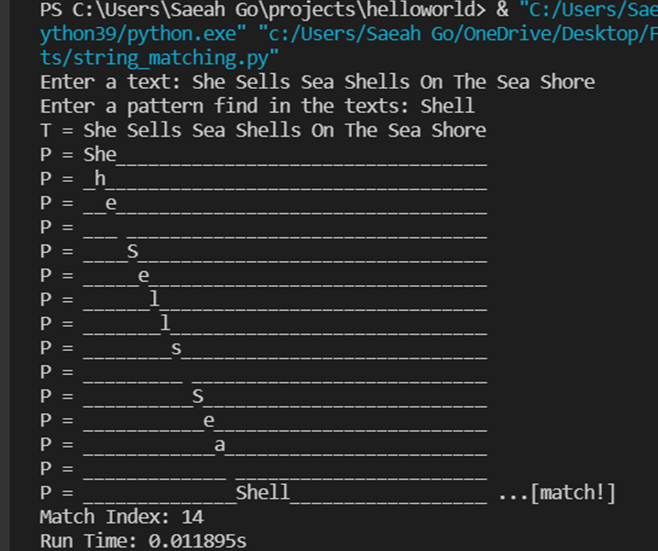
\includegraphics[scale = 0.67]{inputsize 37 average.png} \\
\end{center}
In this case the pattern was found in the fourteenth index, and the running time is about $0.0112$ seconds.
\begin{center}
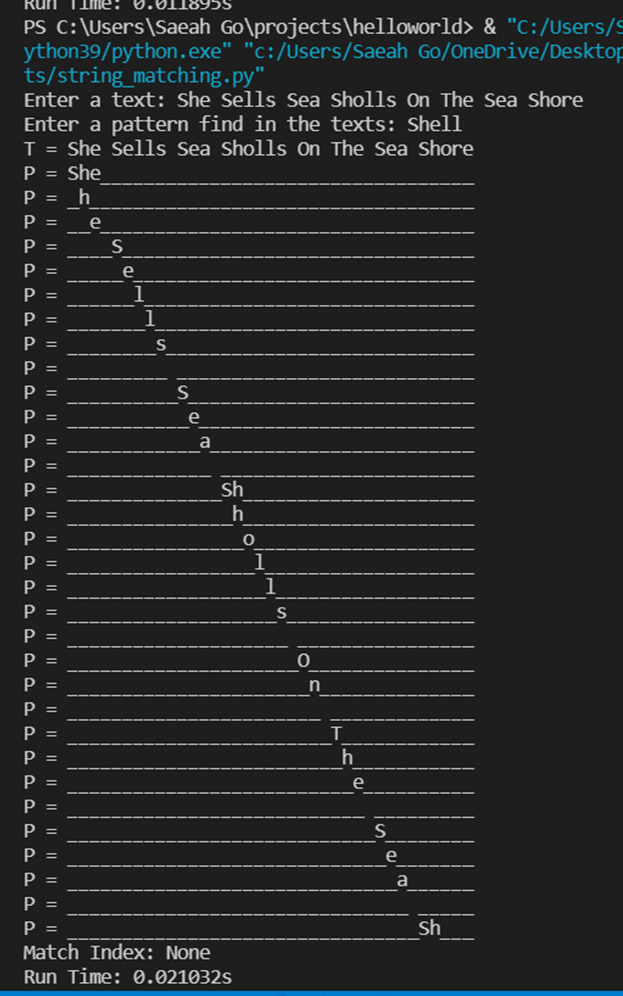
\includegraphics[scale = 0.68]{inputsize 37 worst.png} \\
\end{center}
The last case is the worst case, the input size is really big and we couldn't find the matched string here. Our running time is about $0.02$ seconds.

\section{\textbf{Analysis Results}}
\indent Based on the test performance results, we made a graph in R and we got: \\
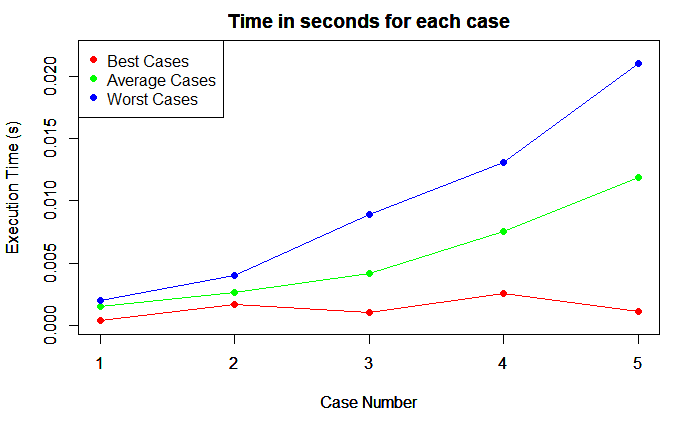
\includegraphics[scale = 0.65]{graph image.png} \\
\indent To explain what the case number denotes briefly, Case 1 indicates the smallest input size case, when the input size was 6. Similarly, Case 5 indicates the biggest input size case, when the input size was 37. As the case number increases the input size increases as well. In the graph we could check that the best cases' running time (the red dot and line) is not much increasing as the input size (text size) gets bigger, since in the best cases (find the matching pattern in our first comparison) we only execute the \textit{j} for loop $m$(the length of pattern) times. For the average (random) cases and worst cases, we could find that both of the graph lines are increasing as the input is gradually bigger. But the worst case graph increases more sharply than the average one, which makes sense because the time complexity of the worst case is $O(nm)$ and the time complexity of the average case is $O(n)$. We know that $O(n) \le O(nm)$. Overall the performance testing went well and we got reasonable values of the running time. We saw the results what we expected before the experiment.

\section{\textbf{Recommendations}}
\indent As I briefly mentioned in the Background part, we compare the pattern in every index of the text in the worst case. It's a lot of comparisons since the time complexity is $O(nm)$. So I recommend using another string matching algorithm, like the KMP algorithm. KMP algorithm (Knuth-Morris-Pratt algorithm) is also a string-searching algorithm. It optimizes the brute force solution by not taking i back when finding a mismatch. And it has an $O(n+m)$ time complexity, which makes it a pretty fast string-searching algorithm. Since the time complexity of the brute force string matching is not the best, I recommend using another better string matching algorithm rather than using the brute force string matching.

\section{\textbf{Appendix 1}} 
\begin{center}
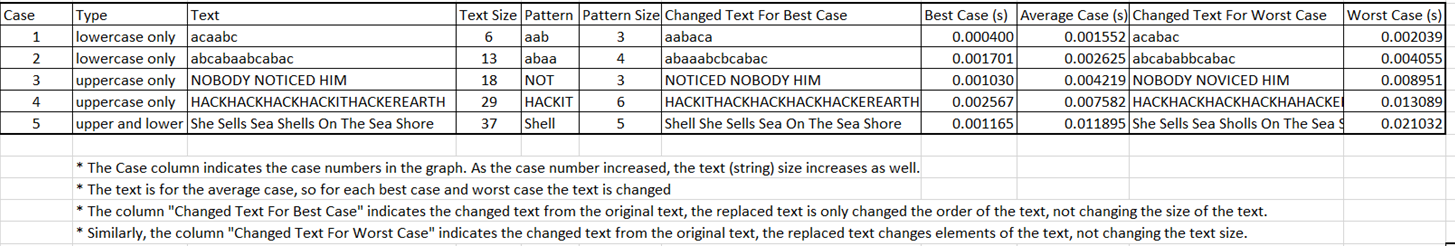
\includegraphics[scale = 0.18]{table} \\
\scriptsize{Table 1}
\end{center}
\indent This table shows the texts we considered in the performance testing. The first column (The Case column) indicates the case number in the graph above in the Analysis Results. More precisely, those are the case numbers which is used when creating a graph. The second column, Text, shows the text string for the average case. We made other two columns for the best and worst case because the text is changed slightly for each case. Pattern column shows the patterns we use for the performance testing. The third column changed. The column ``Changed Text For Best Case" indicates the changed text from the original text, the replaced text is only changed the order of the text, not changing the size of the text. Similarly, the column ``Changed Text For Worst Case" indicates the changed text from the original text, the replaced text changes elements of the text, not changing the text size. 

\begin{center}
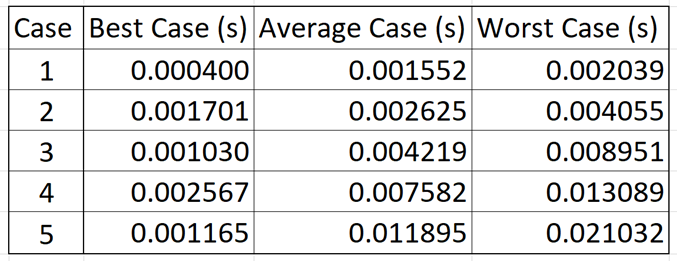
\includegraphics[scale = 0.6]{table2} \\
\scriptsize{Table 2}
\end{center}
\indent We also first included the column Case, as we did in the first table, to make sure this table considered the same cases with the table above. Each case number indicates the same case. The second column, Best Case (s) indicates the running time when we put the string in the Changed Text For Best Case column, and since it's time the unit is seconds, shortly s. Similarly, Average Cases (s) column shows the execution time of random cases. Worst Cases (s) column shows the time it took when we are testing the worst cases. In this table, we can see that every best case value takes the lowest execution time compare to average and worst cases. When we look at the first row, we could see that $0.0004(best) < 0.001552(average) < 0.002039(worst)$. We could observe the same thing in the second, third, fourth, and fifth rows that the value of best case running time is the lowest and the running time of average cases is between its best case and worst case, and the worst case running time is bigger than the average cases' running time. Also as the text sizes ($n$) grow, the execution time for average cases and worst cases grow as well. This result shows what we expected earlier, since the time complexity of Brute Force String Matching is $O(nm)$ when $n$ is the length of text and $m$ is the length of pattern. 

\begin{center}
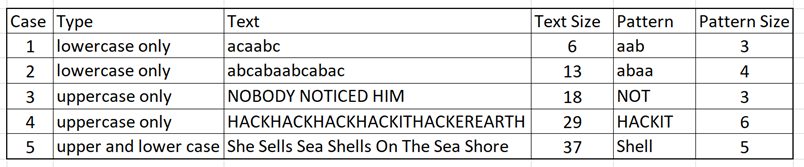
\includegraphics[scale = 0.5]{table3}\\
\scriptsize{Table 3}
\end{center}


This table also includes the Case column. In the Type column, we tried to show the string type, if the string only contains lowercase elements, only contains uppercase elements, or it's a mixture of upper and lower cases. And for the Text column we put the strings we considered for the average cases. Text Size column includes the value of the length of the texts. Pattern column shows the pattern we considered during the experiment, and the Pattern Size column shows the length of the patterns.

\section{\textbf{Appendix 2}}
\indent Our first input (text) is $acaabc$, which input size is 6. The string only consists of all lowercase. We wanted to start from the small amounts of input, so we choose a random string on the internet. \\ 
\indent The second text string is $abcabaabcabac$. Its size is 13, which is more than twice bigger of the input size 6. We thought it's a reasonable length to see the time complexity. This text also only includes lowercase letters, and chooses from the internet. \\
\indent The third string is $NOBODY \; NOTICE \; HIM$. It was an example considered in the textbook we use, thus we choose to consider this in the performance testing. The characteristic of the string is it consists of uppercase letters only and there are some blank spaces (whitespace) unlike the two above cases we considered. The text size is 18, and the pattern size is 3. \\
\indent For the fourth string text, we choose $HACKHACKHACKHACKITHA- CKEREARTH$. Somewhat no make sense sentence, but we wanted to consider a string which has no blank spaces and only consists of upper letteres. Since the length of the text was 29, it was a good middle length to test, that's why we chose this as our fourth test case.\\
\indent For the last text, we chose $She \; Sells \; Sea \; Shells \; On \; The \; Sea \; Shore$. Found this string in a YouTube video that talks about the Brute Force String Matching. This was an example in the video. The text consists of upper and lower case letters, thus the given pattern is also $Shell$ which is different with other four cases. The text length is 37, the most longest among our test cases. \\
\indent For more detailed descriptions of inputs and its size, please check the table 3 in Appendix 1.
\end{document}

